\documentclass{article}

% Language setting
% Replace `english' with e.g. `spanish' to change the document language
\usepackage[english]{babel}

% Set page size and margins
% Replace `letterpaper' with `a4paper' for UK/EU standard size
\usepackage[letterpaper,top=2cm,bottom=2cm,left=3cm,right=3cm,marginparwidth=1.75cm]{geometry}

% Useful packages
\usepackage{amsmath}
\usepackage{graphicx}
\usepackage[colorlinks=true, allcolors=blue]{hyperref}
\usepackage{physics}
\usepackage{tikz}

\title{QFT HW1}
\author{Yonah Weiner 337756787}
\date{June 11, 2024}

\begin{document}
\maketitle
\subsection*{Path Integral Basics}
\subsection*{Solution}
\subsubsection*{(a)}
First we note that:\\
\begin{align*}
      & q_H(t)\ket{q,t}=q\ket{q,t} \\
      & \Rightarrow e^{Ht/\hbar}\hat qe^{-Ht/\hbar}\ket{q,t}=q\ket{q,t}
      \end{align*}
       where $\hat q$ is the Schrodinger picture operator
      \begin{align*}
      & \Rightarrow \hat qe^{-Ht/\hbar}\ket{q,t}=qe^{-Ht/\hbar}\ket{q,t}\\
      & \Rightarrow e^{-Ht/\hbar}\ket{q,t}=\ket{q}
\end{align*}


\begin{equation} \label{eq:s state}
    \Rightarrow \ket{q,t}=e^{Ht/\hbar}\ket{q}
\end{equation}
\noindent
Now we look at the RHS:
\begin{equation*}
    \begin{split}
        \bra{q^F,t_F}q_H(t)\ket{q^I,t_I} & \overbrace{=}^{(\ref{eq:s state})} \bra{q^F}e^{-Ht_F/\hbar}q_H(t)e^{Ht_I/\hbar}\ket{q^I}\\
        &=\bra{q^F}e^{-H(t_F-t)/\hbar}\hat qe^{-H(t - t_I)/\hbar}\ket{q^I}
    \end{split}
\end{equation*}
We can write $\hat q = \int dq\, q \ket{q}\bra{q}$, and plug this into the above to get:
\begin{equation*}
    \begin{split}
        & =\int dq\, q \bra{q^F}e^{-H(t_F-t)/\hbar}\ket{q}\bra{q}e^{-H(t - t_I)/\hbar}\ket{q^I}\\
        & =\int dq \int [Dq] e^{\frac{i}{\hbar}\int_{t}^{t^F}dt'L}\int [Dq] e^{\frac{i}{\hbar}\int_{t^I}^{t}dt'L}q\\
        & =\int [Dq] e^{\frac{i}{\hbar}\int_{t^I}^{t^F}dt'L}q(t)
    \end{split}
\end{equation*}

\subsubsection*{(b)}
For $t>\tilde{t}$:\\
\begin{equation*}
\begin{split}
    \bra{q^F,t_F}q_H(t)q_H(\tilde t)\ket{q^I,t_I} & \overbrace{=}^{(\ref{eq:s state})} 
    \bra{q^F}e^{-Ht_F/\hbar}q_H(t)q_H(\tilde t)e^{Ht_I/\hbar}\ket{q^I}\\
    & = \bra{q^F}e^{-H(t_F-t)/\hbar}\hat q e^{-H(t-\tilde t)/\hbar}\hat qe^{-H(\tilde t - t_I)/\hbar}\ket{q^I}\\
    & = \iint dqdq'\,qq'\bra{q^F}e^{-H(t_F-t)/\hbar}\ket{q}\bra{q}e^{-H(t-\tilde t)/\hbar}\ket{q'}\bra{q'}e^{-H(\tilde t - t_I)/\hbar}\ket{q^I}\\
    & =\iint dq dq' \int [Dq] e^{\frac{i}{\hbar}\int_{t}^{t^F}dt'L}\int [Dq] e^{\frac{i}{\hbar}\int_{\tilde t}^{t}dt'L}\int [Dq] e^{\frac{i}{\hbar}\int_{t^I}^{\tilde t}dt'L}qq'\\
    & =\int [Dq] e^{\frac{i}{\hbar}\int_{t^I}^{t_F}dt'L}q(t)q(\tilde t)
\end{split}
\end{equation*}
Therefore, if $t < \tilde t$, then:
\begin{equation*}
    \begin{split}
       \int [Dq] e^{\frac{i}{\hbar}\int_{t^I}^{t_F}dt'L}q(t)q(\tilde t) & =
       \iint dq dq' \int [Dq] e^{\frac{i}{\hbar}\int_{\tilde t}^{t^F}dt'L}\int [Dq] e^{\frac{i}{\hbar}\int_{t}^{\tilde t}dt'L}\int [Dq] e^{\frac{i}{\hbar}\int_{t^I}^{t}dt'L}qq'\\
       & = \iint dqdq'\,qq'\bra{q^F}e^{-H(t_F-\tilde t)/\hbar}\ket{q}\bra{q}e^{-H(\tilde t- t)/\hbar}\ket{q'}\bra{q'}e^{-H( t - t_I)/\hbar}\ket{q^I}\\
       & = \bra{q^F}e^{-H(t_F-\tilde t)/\hbar}\hat q e^{-H(\tilde t-t)/\hbar}\hat qe^{-H(t - t_I)/\hbar}\ket{q^I}\\
       & = \bra{q^F}e^{-Ht_F/\hbar}q_H(\tilde t)q_H(t)e^{Ht_I/\hbar}\ket{q^I}\\
       & = \bra{q^F,t_F}q_H(\tilde t)q_H(t)\ket{q^I,t_I}
    \end{split}
\end{equation*}
\subsubsection*{(c)}
\begin{equation*}
    \begin{split}
        \dv{t}q_H(t) & =\dv{t}(e^{\frac{i}{\hbar}Ht})\hat qe^{-\frac{i}{\hbar}Ht}+e^{\frac{i}{\hbar}Ht}\hat q\dv{t}(e^{-\frac{i}{\hbar}Ht})\\
        & = \frac{i}{\hbar}He^{\frac{i}{\hbar}Ht}\hat qe^{-\frac{i}{\hbar}Ht}-e^{\frac{i}{\hbar}Ht}\hat q\frac{i}{\hbar}He^{-\frac{i}{\hbar}Ht}\\
    \end{split}
\end{equation*}
because $[H,e^{Ht}]=0$:
\begin{equation*}
    \begin{split}
        & = \frac{i}{\hbar}e^{\frac{i}{\hbar}Ht} H\hat qe^{-\frac{i}{\hbar}Ht}-e^{\frac{i}{\hbar}Ht}\hat q\frac{i}{\hbar}He^{-\frac{i}{\hbar}Ht}\\
        & = \frac{i}{\hbar}e^{\frac{i}{\hbar}Ht}[H,\hat q]e^{-\frac{i}{\hbar}Ht}\\
        & = \frac{i}{\hbar}e^{\frac{i}{\hbar}Ht}[\frac{\hat{p}^2}{2m}+V(q),\hat q]e^{-\frac{i}{\hbar}Ht}\\
        & = \frac{i}{2m\hbar}e^{\frac{i}{\hbar}Ht}[\hat{p}^2,\hat q]e^{-\frac{i}{\hbar}Ht}\\
        & = \frac{i}{2m\hbar}e^{\frac{i}{\hbar}Ht}(\hat p[\hat p,\hat q]+[\hat p,\hat q]\hat p)e^{-\frac{i}{\hbar}Ht}\\
        & = \frac{i}{2m\hbar}e^{\frac{i}{\hbar}Ht}(-2i\hbar \hat p)e^{-\frac{i}{\hbar}Ht}\\
        & = \frac{1}{m}p_H(t)\\
        \Rightarrow & p_H(t)=m\dot{q}_H(t)
    \end{split}
\end{equation*}
\subsubsection*{(d)}

\subsection*{Harmonic Oscillator}
\subsection*{Solution}
For an harmonic oscillator,\\
\begin{equation*}
    q_S=\sqrt{\frac{\hbar}{2\omega}}(a^\dagger + a)
\end{equation*}
\begin{equation*}
    a^\dagger\ket{n}=\sqrt{n+1}\ket{n+1}
\end{equation*}
\begin{equation*}
    a\ket{n}=\sqrt{n}\ket{n-1}
\end{equation*}
\begin{equation*}
    e^{iHt/\hbar}=\sum_{n}e^{i\omega nt}\ket{n}\bra{n}
\end{equation*}

Using these relations, we could calculate:\\
$\bra{0}q(t)q(0)\ket{0}=$$\bra{0}e^{\frac{i}{\hbar} H t}q_Se^{-\frac{i}{\hbar}Ht}q_S\ket{0}=$\\
$=\bra{0}(\sum_{k}e^{i\omega kt}\ket{k}\bra{k})\sqrt{\frac{\hbar}{2\omega}}(a^\dagger + a)(\sum_{n}e^{-i\omega nt}\ket{n}\bra{n})\sqrt{\frac{\hbar}{2\omega}}(a^\dagger + a)\ket{0}$\\
$=(\sqrt{\frac{\hbar}{2\omega}})^2\sum_{k,n}e^{i\omega (k-n)t}\delta_{0 k}\bra{k}(a^\dagger + a)\ket{n}\delta_{n 1} $\\
$=(\sqrt{\frac{\hbar}{2\omega}})^2e^{-i\omega t}\bra{0}(a^\dagger + a)\ket{1}=(\sqrt{\frac{\hbar}{2\omega}})^2e^{-i\omega t}\braket{0}$\\
$=\boxed{\frac{\hbar}{2\omega}e^{-i\omega t}}$\\
If we do a Wick rotation by $t=-i\tau$, we get:\\
$\bra{0}q(\tau)q(0)\ket{0}=\frac{\hbar}{2\omega}e^{-\omega \tau}$\\
which is what we saw in class.\\\\
Now we will use residue calculus and calculate:\\
$\int_{-\infty}^{\infty}\frac{dp}{2\pi}\frac{e^{ip\tau}}{p^2+\omega^2}=\oint_\gamma\frac{dp}{2\pi}\frac{e^{ip\tau}}{p^2+\omega^2}$\\
where $\gamma$ is the path in complex space which looks like:\\
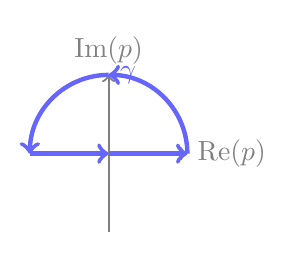
\begin{tikzpicture}
% draw axis
    \draw[gray, thick][->] (-1,0) -- (1,0) node [right] {$\Re(p)$};
    \draw[gray, thick][->] (0,-1) -- (0,1) node [above] {$\Im(p)$};
    %draw contour
    \draw[blue!60, ultra thick, ->] (-1,0) -- (0,0) ;
    \draw[blue!60, ultra thick, ->] (0,0) -- (1,0);
    \draw[blue!60, ultra thick, ->] (1,0) arc (0:90:1) node [below, right] {$\gamma$};
    \draw[blue!60, ultra thick, ->] (0,1) arc (90:180:1);
\end{tikzpicture}

The contour is at the limit as the radius of the semicircle goes to infinity. We chose the semicircle with $\Im[p]>0$ so that the contribution from the arc goes to zero leaving us only with the contribution from the real axis. This works only for $\tau > 0$ There are poles at $p=\pm i\omega$. The residue from our contour is:\\
$Res(\frac{1}{2\pi}\frac{e^{ip\tau}}{p^2+\omega^2})= \lim_{p\rightarrow i\omega}(p-i\omega)\frac{1}{2\pi}\frac{e^{ip\tau}}{p^2+\omega^2}=$$\lim_{p\rightarrow i\omega}\frac{1}{2\pi}\frac{e^{ip\tau}}{p+i\omega}=$$\frac{1}{4\pi}\frac{e^{-\omega\tau}}{i\omega}$\\
Now we plug this into the residue theorem and get:\\
$\int_{-\infty}^{\infty}\frac{dp}{2\pi}\frac{e^{ip\tau}}{p^2+\omega^2}=\oint_\gamma\frac{dp}{2\pi}\frac{e^{ip\tau}}{p^2+\omega^2}=2\pi i\sum Res(\frac{1}{2\pi}\frac{e^{ip\tau}}{p^2+\omega^2})=2 \pi i \frac{1}{2\pi}\frac{e^{-\omega\tau}}{2i\omega}=\frac{e^{-\omega\tau}}{2\omega}$\\
Note that here we assumed $\tau > 0$. When $\tau < 0$, we must choose the contour which looks like: 

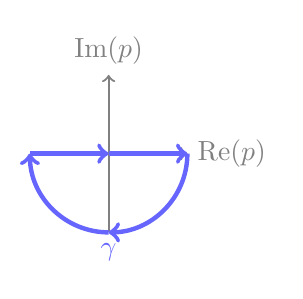
\begin{tikzpicture}
% draw axis
    \draw[gray, thick][->] (-1,0) -- (1,0) node [right] {$\Re(p)$};
    \draw[gray, thick][->] (0,-1) -- (0,1) node [above] {$\Im(p)$};
    %draw contour
    \draw[blue!60, ultra thick, ->] (-1,0) -- (0,0) ;
    \draw[blue!60, ultra thick, ->] (0,0) -- (1,0);
    \draw[blue!60, ultra thick, ->] (1,0) arc (0:-90:1) node [below] {$\gamma$};
    \draw[blue!60, ultra thick, ->] (0,-1) arc (-90:-180:1);
\end{tikzpicture}

this way the contribution of the arc goes to zero. In this case the pole is at $-i\omega$, which changes the residue to:\\
$\frac{-1}{4\pi}\frac{e^{\omega\tau}}{i\omega}$. In addiction we notice that our contour is clockwise, which gives us a minus in front of the integral. In total our integral is:
$\int_{-\infty}^{\infty}\frac{dp}{2\pi}\frac{e^{ip\tau}}{p^2+\omega^2}=\frac{e^{\omega\tau}}{2\omega}$\\
Putting these answers together for all $\tau$, we get:\\
$\boxed{\int_{-\infty}^{\infty}\frac{dp}{2\pi}\frac{e^{ip\tau}}{p^2+\omega^2}=\frac{e^{\omega|\tau|}}{2\omega}}$\\
\subsection*{Wick's contractions basics}
Show that:
\begin{equation} \label{eq:zed}
\mathcal{Z}[J]=\int d^N q e^{-\frac{1}{2} q^T M q+J \cdot q}=(2 \pi)^{\frac{N}{2}}(\operatorname{det} M)^{-\frac{1}{2}} e^{\frac{1}{2} J^T M^{-1} J} 
\end{equation}
\subsection*{Solution}
$M$ is diagonal, so it can be written as $M_{ij}=\delta_{ij}\lambda_i$ (no sum on i). We can rewrite the LHS of equation (\ref{eq:zed}) as:\\
$\int d^N q e^{-\frac{1}{2} q^T M q+J \cdot q}=\int d^N q e^{-\frac{1}{2} \sum_i \lambda_i q_i^2+J_iq_i}= \Pi_i \int d^N q e^{-\frac{1}{2} \lambda_i q_i^2+J_iq_i}$\\
By completing the square, this becomes:\\
$=\Pi_i e^{\frac{1}{2}J^2_i/\lambda_i}\int d^N q e^{-\frac{\lambda_i}{2}(q_i-J_i/\lambda_i)^2}$\\
we compute this as a Gaussian:\\
$=\Pi_i e^{\frac{1}{2}J^2_i/\lambda_i}(2\pi/\lambda_i)^{1/2}=(2\pi)^{\frac{N}{2}}(\Pi_i \frac{1}{\lambda_i})(\Pi_i e^{\frac{1}{2}J^2_i/\lambda_i})=(*)$. \\
We note that $M^{-1}_{ij}=\delta_{ij}\frac{1}{\lambda_i}$ (no sum on i), and the determinant is the product of the eigenvalues: $\det M =\Pi_i \frac{1}{\lambda_i}$. Plugging this into $(*)$:\\
$=(2\pi)^{\frac{N}{2}}(\det (M^{-1}))^{\frac{1}{2}}e^{\sum_{i,j} \frac{1}{2}J_i\delta_{ij}(\frac{1}{\lambda_i})J_j}=$$(2\pi)^{\frac{N}{2}}(\det M)^{-\frac{1}{2}}e^{ \frac{1}{2}J^T(M^{-1})J}$.\\
which is what we wanted to prove.\\\\
Now we wish to show:\\
\begin{equation}
\frac{1}{Z[0]} \int d^N q e^{-\frac{1}{2} q^T M q} F(q)=\left.\frac{1}{Z[0]} F\left(\frac{\partial}{\partial J}\right) Z[J]\right|_{J=0} .
\end{equation}
We can expand $F(q)$ as a Taylor series in $q$:\\
$F(\mathbf{q})=\sum_{n=0}^{\infty} \frac{1}{n!}\frac{\partial^{(n)}F}{\partial \mathbf{q}^n}|_{\mathbf{q}=0}$
\subsection*{Anharmonic Oscilator}
\begin{equation*}
    H=\frac{1}{2}p^2+\frac{1}{2}q^2+\frac{1}{4!}gq^4
\end{equation*}
\subsection*{(a)}
\subsection*{Solution}
We want to compute the propagator:\\
\begin{equation} \label{eq:prop}
    \langle q(\tau_2)q(\tau_1)\rangle=\frac{\int [Dq]e^{\int_{\tau_1}^{\tau_2}d\tau'L_E}q(\tau_1)q(\tau_2)}{\int [Dq]e^{\int_{\tau_1}^{\tau_2}d\tau'L_E}}
\end{equation}
In our case $L_E=-(\frac{1}{2}(\partial_\tau q)^2+\frac{1}{2}q^2+\frac{1}{4!}gq^4)$. We label $L_E'=-(\frac{1}{2}(\partial_\tau q)^2+\frac{1}{2}q^2)$, and we can rewrite (\ref{eq:prop}) as:
\begin{equation} 
\begin{split}
    \langle q(\tau_2)q(\tau_1)\rangle & 
    =\frac{\int [Dq]e^{\int_{\tau_1}^{\tau_2}d\tau'L_E'}e^{\int_{\tau_1}^{\tau_2}d\tau' (-\frac{1}{4!}gq^4)}q(\tau_1)q(\tau_2)}{\int [Dq]e^{\int_{\tau_1}^{\tau_2}d\tau'L_E'}e^{\int_{\tau_1}^{\tau_2}d\tau' (-\frac{1}{4!}gq^4)}}\\
    &=\frac{1}{\mathcal{Z}_g}\int [Dq]e^{\int_{\tau_1}^{\tau_2}d\tau'L_E'}e^{\int_{\tau_1}^{\tau_2}d\tau' (-\frac{1}{4!}gq^4)}q(\tau_1)q(\tau_2)
\end{split}
\end{equation}
We can expand the exponent containing the anharmonic term: 
\begin{equation*}
    e^{\int_{\tau_1}^{\tau_2}d\tau' (-\frac{1}{4!}gq^4)}=
    \sum_{n=0}^{\infty}\frac{1}{n!}(-\frac{1}{4!}g)^n\overbrace{\idotsint}^n d\tau_1'\dots d\tau_n' q(\tau_1')^4\dots q(\tau_n')^4
\end{equation*}
We are only interested in the n=2 terms:
\begin{equation*}
    e^{\int_{\tau_1}^{\tau_2}d\tau' (-\frac{1}{4!}gq^4)}=
    \sum_{n=0}^{\infty}\frac{1}{n!}(-\frac{1}{4!}g)^n\overbrace{\idotsint}^n d\tau_1'\dots d\tau_n' q(\tau_1')^4\dots q(\tau_n')^4
\end{equation*}
We plug this into the numerator of (\ref{eq:anharmonic prop}) and get:
\begin{equation*}
   \langle q(\tau_2)q(\tau_1) \rangle_{\text{anharmonic}} = \frac{\mathcal{Z}_0}{\mathcal{Z}_g}\mathcal  \sum_{n=0}^{\infty}\frac{1}{n!}(-\frac{1}{4!}g)^n\overbrace{\idotsint}^n d\tau_1'\dots d\tau_n' \langle q(\tau_1)q(\tau_2) q(\tau_1')^4\dots q(\tau_n')^4\rangle_{\text{harmonic}} 
\end{equation*}
where
\begin{equation*}
   \frac{\mathcal{Z}_g}{\mathcal{Z}_0} = \sum_{n=0}^{\infty}\frac{1}{n!}(-\frac{1}{4!}g)^n\overbrace{\idotsint}^n d\tau_1'\dots d\tau_n' \langle  q(\tau_1')^4\dots q(\tau_n')^4\rangle_{\text{harmonic}} 
\end{equation*}
\end{document}